\section{View Cleaning: Scale View as Dirty Data \cite{krishnan2015svc}}



In follow-up work, we explored the generalization of SampleClean.
Suppose the relation $R$ is in fact a derived relation $V$ of an underlying dirty database $D$.
We explored how we can efficiently apply a data cleaning operation to a sample of $V$.
This extension has an important application in approximate Materialized View maintenance, where we model a stale Materialized View as dirty data, and the maintenance procedure as cleaning.  

\subsection{Motivation}
There has been significant research on fast MV maintenance algorithms, most recently DBToaster \cite{DBLP:journals/vldb/KochAKNNLS14} which uses SQL query compilation and higher-order maintenance.
However, even with these optimizations, some materialized views are computationally difficult to maintain and will have maintenance costs that can grow with the size of data (e.g, correlated aggregate in a sub-query).
When faced with such challenges, it is common to batch updates to amortize maintenance overheads and add flexibility to scheduling.
Like dirty data, any amount of staleness can lead to erroneous query results where the user has no idea about the magnitude or the scope of query error. 
Thus, we explore how samples of ``clean" (up-to-date) data can be used for improved query processing on MVs without incurring the full cost of maintenance.

\subsection{Notation and Definitions}\label{notation}
\svc returns a bounded approximation for aggregate queries on stale MVs for a flexible additional maintenance cost.

\noindent \textbf{Materialized View:} Let $\mathcal{D}$ be a database which is a collection of relations $\{R_i\}$. 
A \emph{materialized view} $V$ is the result of applying a \emph{view definition} to $\mathcal{D}$. 
View definitions are composed of standard relational algebra expressions: Select ($\sigma_{\phi}$), Project ($\Pi$), Join ($\bowtie$), Aggregation ($\gamma$), Union ($\cup$), Intersection ($\cap$) and Difference ($-$). 

\vspace{0.5em}

\noindent \textbf{Primary Key:} We assume that each of the base relations has a \emph{primary key}. If this is not the case, we can always add an extra column that assigns an increasing sequence of integers to each record. 
This primary key is formally a subset of attributes $u \subseteq \{a_1,a_2,...,a_k\}$ such that all $s \in V(u)$ are unique.

\vspace{0.5em}

\noindent \textbf{Staleness:} For each relation $R_i$ there is a set of insertions $\Delta R_i$ (modeled as a relation)
and a set of deletions $\nabla R_i$.
An ``update'' to $R_i$ can be modeled as a deletion and then an insertion.
We refer to the set of insertion and deletion relations as ``delta relations", denoted by $\partial \mathcal{D}$:
\[
	\partial \mathcal{D} = \{\Delta R_1,...,\Delta R_k\} \cup \{\nabla R_1,...,\nabla R_k\}
\]
A view $S$ is considered \emph{stale} when there exist insertions or deletions to any of its base relations.
This means that at least one of the delta relations in $\partial \mathcal{D}$ is non-empty.

\vspace{0.5em}

\noindent \textbf{Maintenance:} There may be multiple ways (e.g., incremental maintenance or recomputation) to maintain a view $V$, and we denote the up-to-date view as $V'$.
We formalize the procedure to maintain the view as a \emph{maintenance strategy} $\mathcal{M}$.
A maintenance strategy is a relational expression the execution of which will return $V'$.
It is a function of the database $\mathcal{D}$, the stale view $V$, and all the insertion and deletion relations $\partial \mathcal{D}$. 
In this work, we consider maintenance strategies composed of the same relational expressions as materialized views described above.
\[
V' = \mathcal{M}(V,\mathcal{D}, \partial D)
\]

\vspace{0.5em}

\noindent \textbf{Staleness as Data Error:} The consequences of staleness are incorrect, missing, and superfluous rows. 
Formally, for a stale view $V$ with primary key $u$ and an up-to-date view $V'$:
\begin{itemize}[noitemsep] \sloppy
	\item \textbf{Incorrect: } Incorrect rows are the set of rows (identified by the primary key) that are updated in $V'$. For $v \in V$, let $v(u)$ be the value of the primary key. An incorrect row is one such that there exists a $v' \in V'$ with $v'(u) = V(u)$ and $v \ne v'$.
	\item \textbf{Missing: } Missing rows are the set of rows (identified by the primary key) that exist in the up-to-date view but not in the stale view. For $v' \in V'$, let $v'(u)$ be the value of the primary key. A missing row is one such that there does not exist a $v \in V$ with $v(u) = v'(u)$.
	\item \textbf{Superfluous: } Superfluous rows are the set of rows (identified by the primary key) that exist in the stale view but not in the up-to-date view. For $v \in V$, let $v(u)$ be the value of the primary key. A superfluous row is one such that there does not exist a $v' \in V'$ with $v(u) = v'(u)$.
\end{itemize}

\vspace{0.5em}

\noindent \textbf{Uniform Random Sampling:}
We define a sampling ratio $m\in [0,1]$ and for each row in a view $V$, we include it into a sample with probability $m$.
The relation $S$ is a \emph{uniform sample} of $V$ if
\[\text{(1) } \forall s \in S : s \in V\text{;~~~~~ (2) }Pr(s_1 \in S) =  Pr(s_2 \in S) = m.\]

\vspace{0.5em}

We say a sample is \emph{clean} if and only if it is a uniform random sample of the up-to-date view $V'$. 

\subsection{Problem Setup}
Formally, the workflow of \svc is:\vspace{-0.5em}
\begin{enumerate}[noitemsep]
\item We are given a view $V$.
\item $\mathcal{M}$ defines the maintenance strategy that updates $V$ at each maintenance period.
\item The view $V$ is stale between periodic maintenance, and the up-to-date view should be $V'$.
\item \emph{(Problem 1. Stale Sample View Cleaning)} We find an expression $\mathcal{C}$ derived from $\mathcal{M}$ 
that cleans a uniform random sample of the stale view $V$ to produce a ``clean" sample of the up-to-date
view $S_{clean}$.
\item \emph{(Problem 2. Query Result Estimation)} Given an aggregate query $q$ and the state query result $q(S)$, we use $S_{clean}$ and $S$ to estimate the up-to-date result.
\end{enumerate} 

\jn{The problem definition is a little messed up. ``Stale View Cleaning" should be problem 1; there's no problem 2.}

\noindent\textbf{Stale Sample View Cleaning: }
The first problem addressed by \svc is how to clean a sample of the stale materialized view.
\begin{problem}[Stale View Cleaning]\sloppy
We are given a stale view $S$, a sample of this stale view $S$ with ratio $m$, the maintenance strategy $\mathcal{M}$, the base relations $\mathcal{D}$, and
the insertion and deletion relations $\partial \mathcal{D}$.
We want to find a relational expression $\mathcal{C}$ such that:
\[
V' = \mathcal{C}(S,\mathcal{D},\partial \mathcal{D}),
\]
where $V'$ is a sample of the up-to-date view with ratio $m$. 
\end{problem}

\noindent\textbf{Query Result Estimation: }
The second problem addressed in this paper is query result estimation.
This problem can be addressed with the direct estimation and correction techniques 
described previously.

\subsection{Cleaning a Sample View}
To setup the problem, we first consider two naive solutions to this problem that will not work. 
We could trivially apply $\mathcal{M}$ to the entire stale view $S$ and update it to $V'$, and then sample.
While the result is correct according to our problem formulation, it does not save us on any computation for maintenance.
We want to avoid materialization of up-to-date rows outside of the sample. 
However, the naive alternative solution is also flawed. 
For example, we could just apply $\mathcal{M}$ to the stale sample $S$ and a sample of the delta relations $\widehat{\partial \mathcal{D}}$. 
The challenge is that $\mathcal{M}$ does not always commute with sampling.

\vspace{0.5em} 

\noindent\textbf{Provenance: } To address the commutativity problem, we need to ensure that for each $s \in V'$ all contributing rows in subexpressions to $s$ are also sampled. 
Provenance, also termed lineage, has been an important tool in the analysis of materialized views \cite{DBLP:journals/vldb/CuiW03} and in approximate query processing \cite{DBLP:conf/sigmod/ZengGMZ14}. 
We recursively define a set of primary keys for all relations in the expression tree to define tuple provenance:
\begin{definition} [Primary Key Generation]\label{pk}
For every relational expression $R$, we define the primary key attribute(s) of every expression to be:
\begin{itemize}[noitemsep]
\item Base Case: All relations (leaves) must have an attribute $p$ which is designated as a primary key. 
\item $\sigma_{\phi}(R)$: Primary key of the result is the primary key of R 
\item $\Pi_{(a_1,...,a_k)}(R)$: Primary key of the result is the primary key of R. The primary key must always be included in the projection.
\item $\bowtie_{\phi (r1,r2)}(R_1,R_2)$: Primary key of the result is the tuple of the primary keys of $R_1$ and $R_2$. 
\item $\gamma_{f,A}(R)$: The primary key of the result is the group by key $A$ (which may be a set of attributes).
\item $R_1 \cup R_2$: Primary key of the result is the union of the primary keys of $R_1$ and $R_2$
\item $R_1 \cap R_2$: Primary key of the result is the intersection of the primary keys of $R_1$ and $R_2$
\item $R_1 - R_2$: Primary key of the result is the primary key of $R_1$
\end{itemize}
For every node at the expression tree, these keys are guaranteed to uniquely identify a row.
\end{definition}
These rules define a constructive definition that can always be applied for our defined relational expressions. 

\vspace{0.5em} 

\noindent\textbf{Hashing: } The primary keys allow us to determine the set of rows that contribute to a row $r$ in a derived relation.
If we have a deterministic way of mapping a primary key to a Boolean, we can ensure that all contributing rows are also sampled. 
To achieve this we use a hashing procedure.
Let us denote the hashing operator $\eta_{a, m}(R)$. 
For all tuples in R, this operator applies a hash function whose range is $[0,1]$ to primary key $a$ (which may be a set) and selects those records with hash less than or equal to $m$.
To avoid materializing extra rows, we push down the hashing operator through the expression tree:
\begin{definition}[Hash push-down]
For a derived relation $R$, the following rules can be applied to push $\eta_{a, m}(R)$ down the expression tree. 
\begin{itemize}[noitemsep]
\item $\sigma_{\phi}(R)$: Push $\eta$ through the expression.  
\item $\Pi_{(a_1,...,a_k)}(R)$: Push $\eta $ through if $a$ is in the projection.
\item $\bowtie_{\phi (r1,r2)}(R_1,R_2)$: No push down in general. There are special cases below where push down is possible.
\item $\gamma_{f,A}(R)$: Push $\eta $ through if $a$ is in the group by clause $A$.
\item $R_1 \cup R_2$: Push $\eta $ through to both $R_1$ and $R_2$
\item $R_1 \cap R_2$: Push $\eta $ through to both $R_1$ and $R_2$
\item $R_1 - R_2$: Push $\eta $ through to both $R_1$ and $R_2$
\end{itemize}
\end{definition}

\noindent \textbf{Special Case of Joins: }
In general, a join $R \bowtie S$ blocks the push-down of the hash operator $\eta_{a, m}(R)$ since $a$ possibly consists of attributes in both $R$ and $S$.
However, when there is a constraint that enforces these attributes are equal then push-down is possible.

\emph{Foreign Key Join. } If we have a join with two foreign-key relations $R_1$ (fact table with foreign key $a$) and $R_2$ (dimension table with primary key $b \subseteq a$) and we are sampling the key $a$, then we can push the sampling down to $R_1$. This is because we are guaranteed that for every $r_1\in R_1$ there is only one $r_2 \in R_2$. 

\emph{Equality Join. } If the join is an equality join and $a$ is one of the attributes in the equality join condition $R_1.a = R_2.b$, then $\eta$ can be pushed down to both $R_1$ and $R_2$. On $R_1$ the pushed down operator is $\eta_{a, m}(R_1)$ and on $R_2$ the operator is $\eta_{b, m}(R_2)$.

\vspace{0.5em} 

\noindent \textbf{Efficient View Cleaning: }
If we apply the hashing operator to $\mathcal{M}$, we can get an optimized cleaning expression $\mathcal{C}$ that avoids materializing unnecessary rows. 
When applied to a stale sample of a view $S$, the database $\mathcal{D}$, and the delta relations $\partial \mathcal{D}$, it produces an up-to-date sample with sampling ratio $m$:
\[
V' = \mathcal{C}(S,\mathcal{D},\partial \mathcal{D})
\]
Thus, it addresses Problem 1, and with the materialized sample of up-to-date rows, we can apply the direct estimates and corrections in the previous section to estimate the result bounded in confidence intervals.



\subsection{Results: Video Streaming Log Analysis}
We evaluate \svc on Apache Spark~1.1.0 with 1TB of logs from a video streaming company, Conviva \cite{conviva}.
This is a denormalized user activity log corresponding to video views and various metrics such as data transfer rates, and latencies.
Accompanying this data is a four month trace of queries in SQL.
We identified 8 common summary statistics-type queries that calculated engagement and error-diagnosis metrics.
These 8 queries defined the views in our experiments.
We populated these view definitions using the first 800GB of user activity log records.  
We then applied the remaining 200GB of user activity log records as the updates (i.e., in the order they arrived) in our experiments.
We generated aggregate random queries over this view by taking either random time ranges or random subsets of customers.

\begin{figure}[t]
\centering
 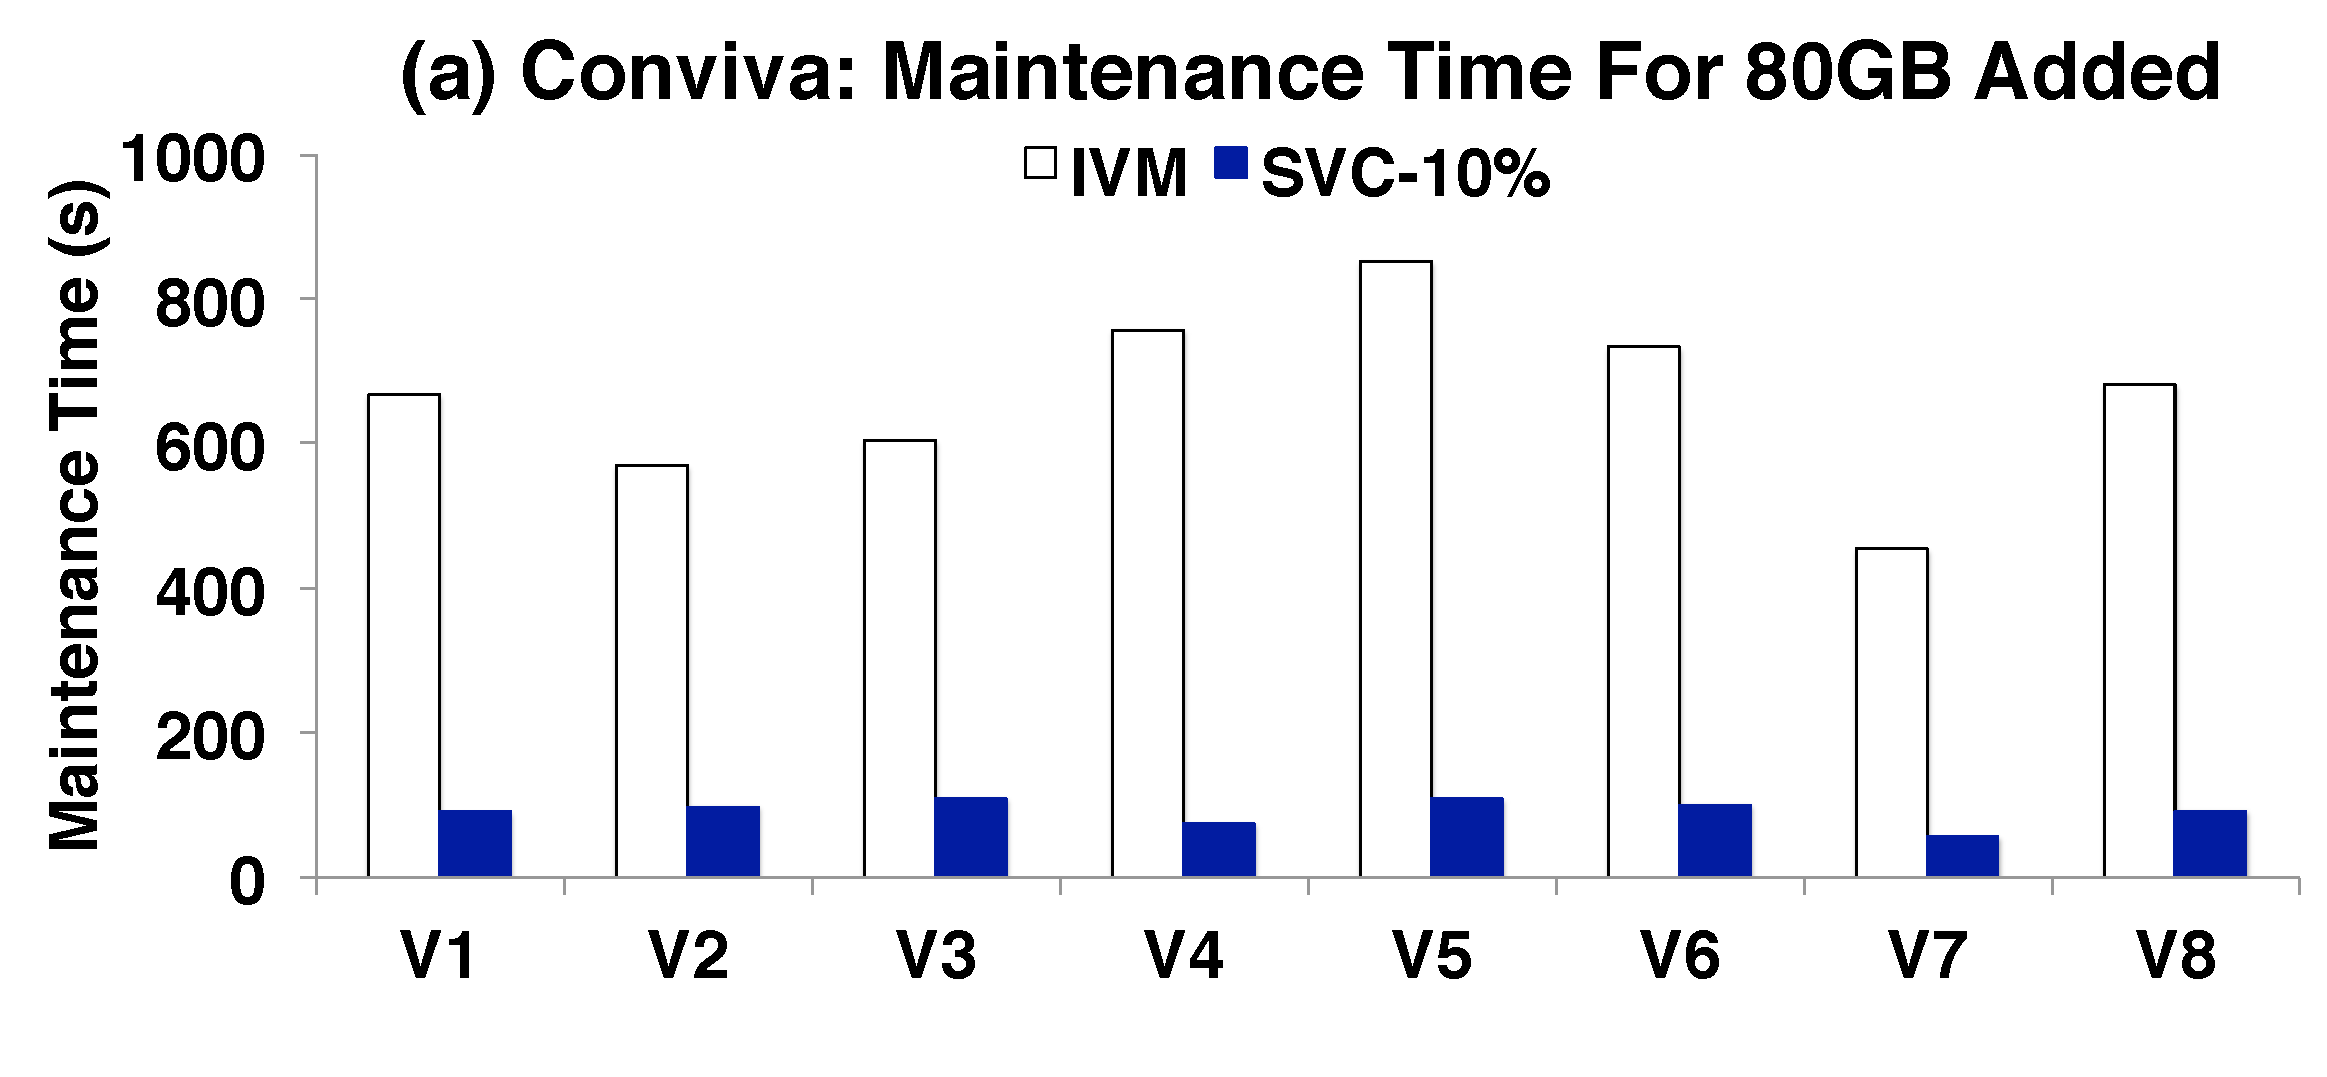
\includegraphics[scale=0.16]{figs/con_3.pdf}
 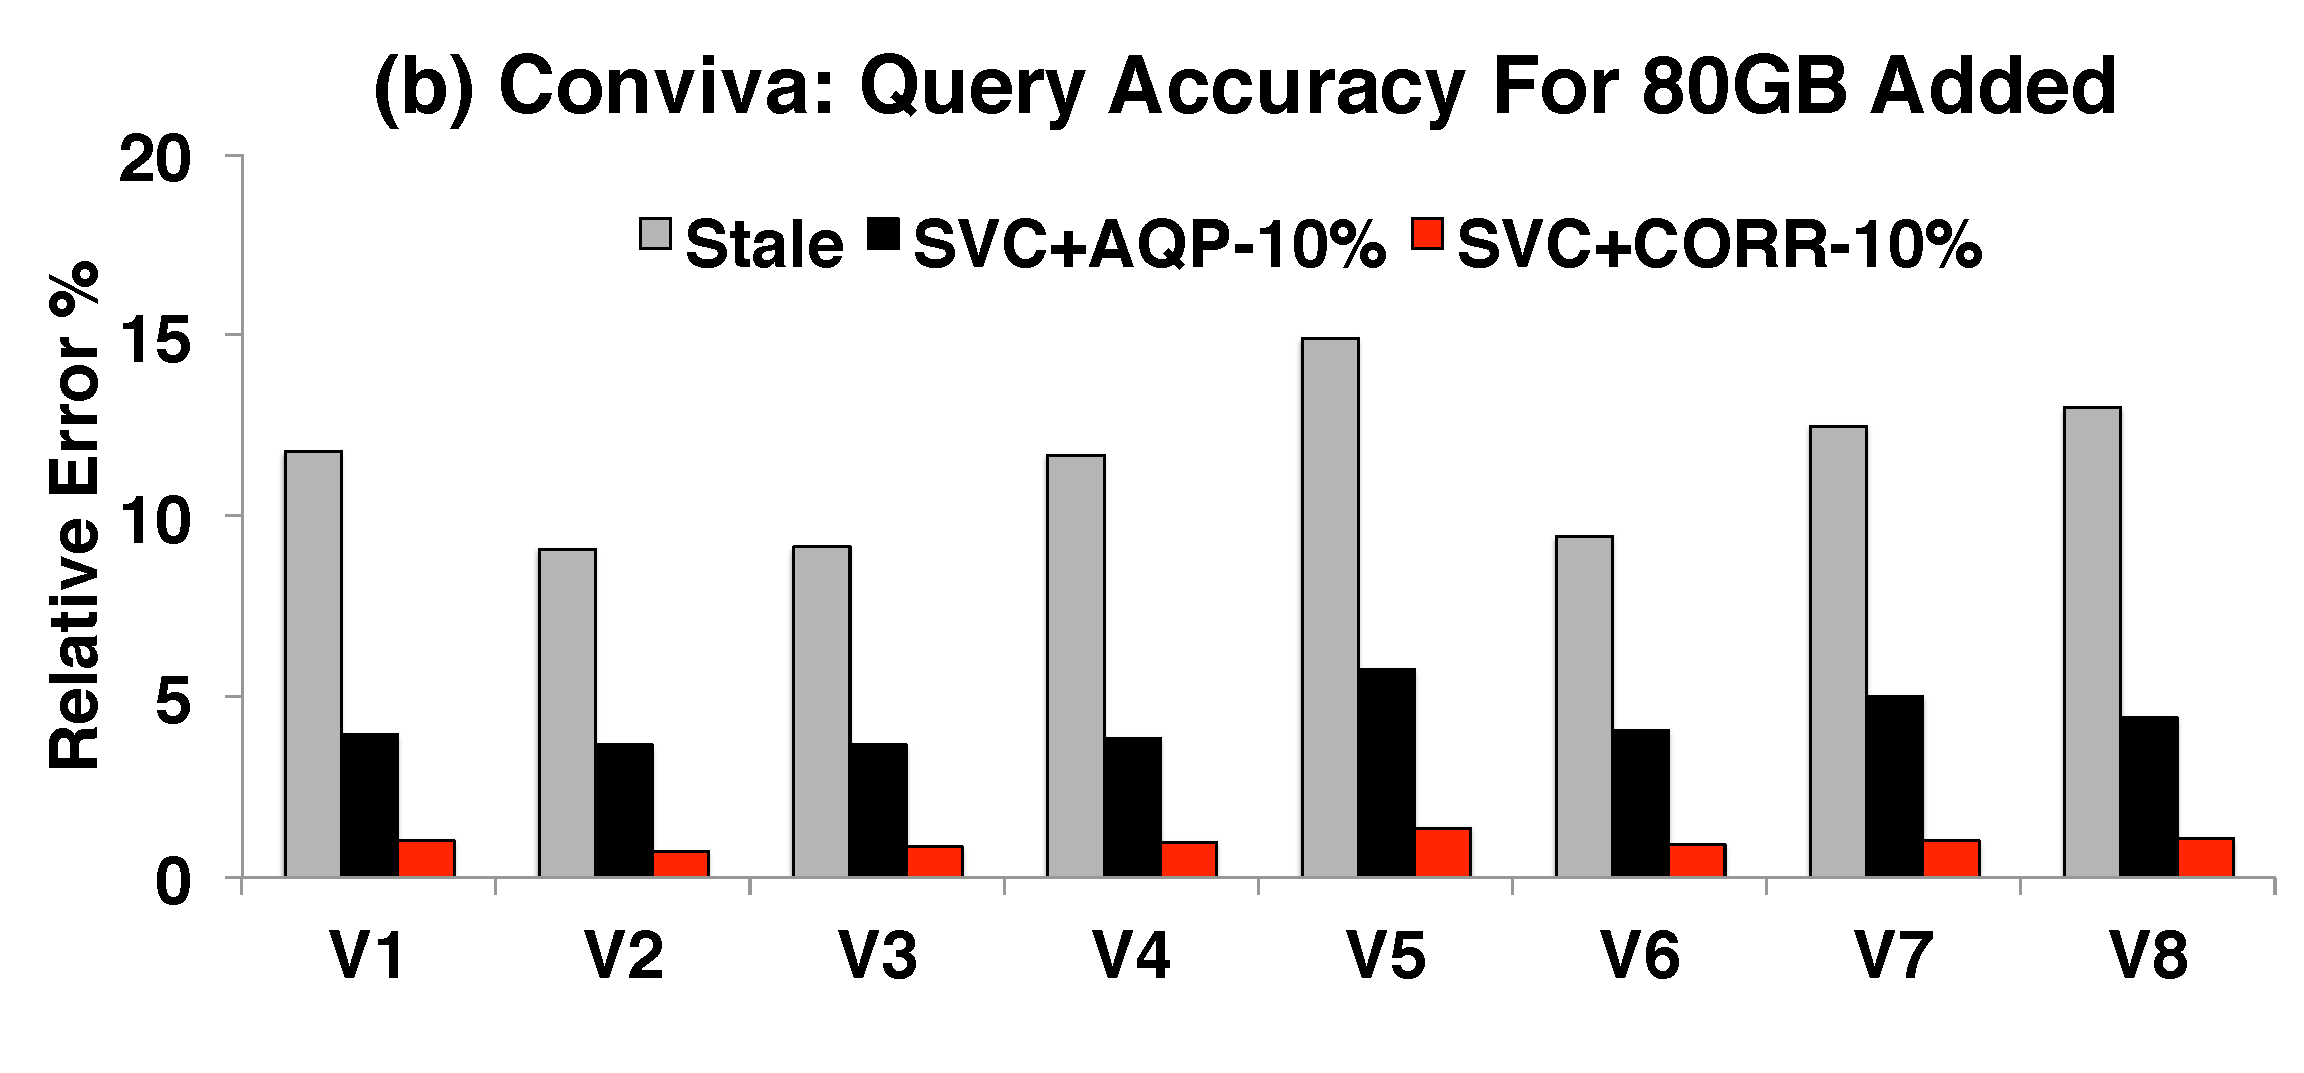
\includegraphics[scale=0.16]{figs/con_4.pdf} \vspace{-1.5em}
 \caption{(a) We compare the maintenance time of \svc with a 10\% sample and full incremental maintenance, and find that as with TPCD \svc saves significant maintenance time. (b) We also evaluate the accuracy of the estimation techniques. \label{conv-1}}\vspace{-1.5em}
\end{figure}

\jn{Explain what IVM, SVC-10\%, Stale, SVC+AQP-10\%, and SVC+CORR-10\% stand for. }

In Figure \ref{conv-1}(a), we show that on average over all the views, \svc-10\% gives a 7.5x speedup.
For one of the views full incremental maintenance takes nearly 800 seconds, even on a 10-node cluster, which is a very significant cost.
In Figure \ref{conv-1}(b), we show that \svc also gives highly accurate results with an average error of 0.98\%.
These results show consistency with our results on the synthetic datasets.
This experiment highlights a few salient benefits of \svc: (1) sampling is a relatively cheap operation and the relative speedups in a single node and distributed environment are similar, (2) for analytic workloads like Conviva (i.e., user engagement analysis) a 10\% sample gives results with 99\% accuracy, and (3) savings are still significant in systems like Spark that do not support selective updates.

